\documentclass{beamer}

\usetheme{Madrid}
\usepackage{graphicx}
\usepackage{multimedia}
\usepackage{tabularx}
\usepackage{subfig}

\title{Multiprojector seamless tiled display}
\author{Pranav Kant Gaur}
\institute{Graphics and Visualization section}

\date{\today}

\begin{document}

\begin{frame}
\titlepage
\end{frame}

%//////////////////////////////////////////////////////////////////////////////////////////////////////////////////////////////////
\begin{frame}
\frametitle{Agenda}
\begin{enumerate}
\item The Problem 
\item Motivation
\item Existing solutions
\item Why not a commercial system?
\item Solution overview
\item System setup
\item Algorithm 
\item Novelity
\item Results
\item Issues
\end{enumerate}
\end{frame}
%//////////////////////////////////////////////////////////////////////////////////////////////////////////////////////////////////

%//////////////////////////////////////////////////////////////////////////////////////////////////////////////////////////////////
\begin{frame}
\frametitle{The Problem}
%Given an arbitrarily arranged grid of projectors projecting at arbitrary positions onto the screen, find the region in each projector image buffer where if the original image is mapped onto will result in a seamless rectangular projection region on the screen.\newline
%In short, 
%ADD UNALIGNED=> ALIGNED ??????????????????????
%Given an arbitrarily arranged grid of projectors projecting at arbitrary positions onto the screen, how to manipulate each projector image so that projected content is \textit{seamless} across the adjacent projectors. \textb{ADD FIGURE!!!!}
We want to create a large image on the projection screen by combining images projected by multiple projectors \textbf{ADD FIGURE!!!!}

\begin{figure}
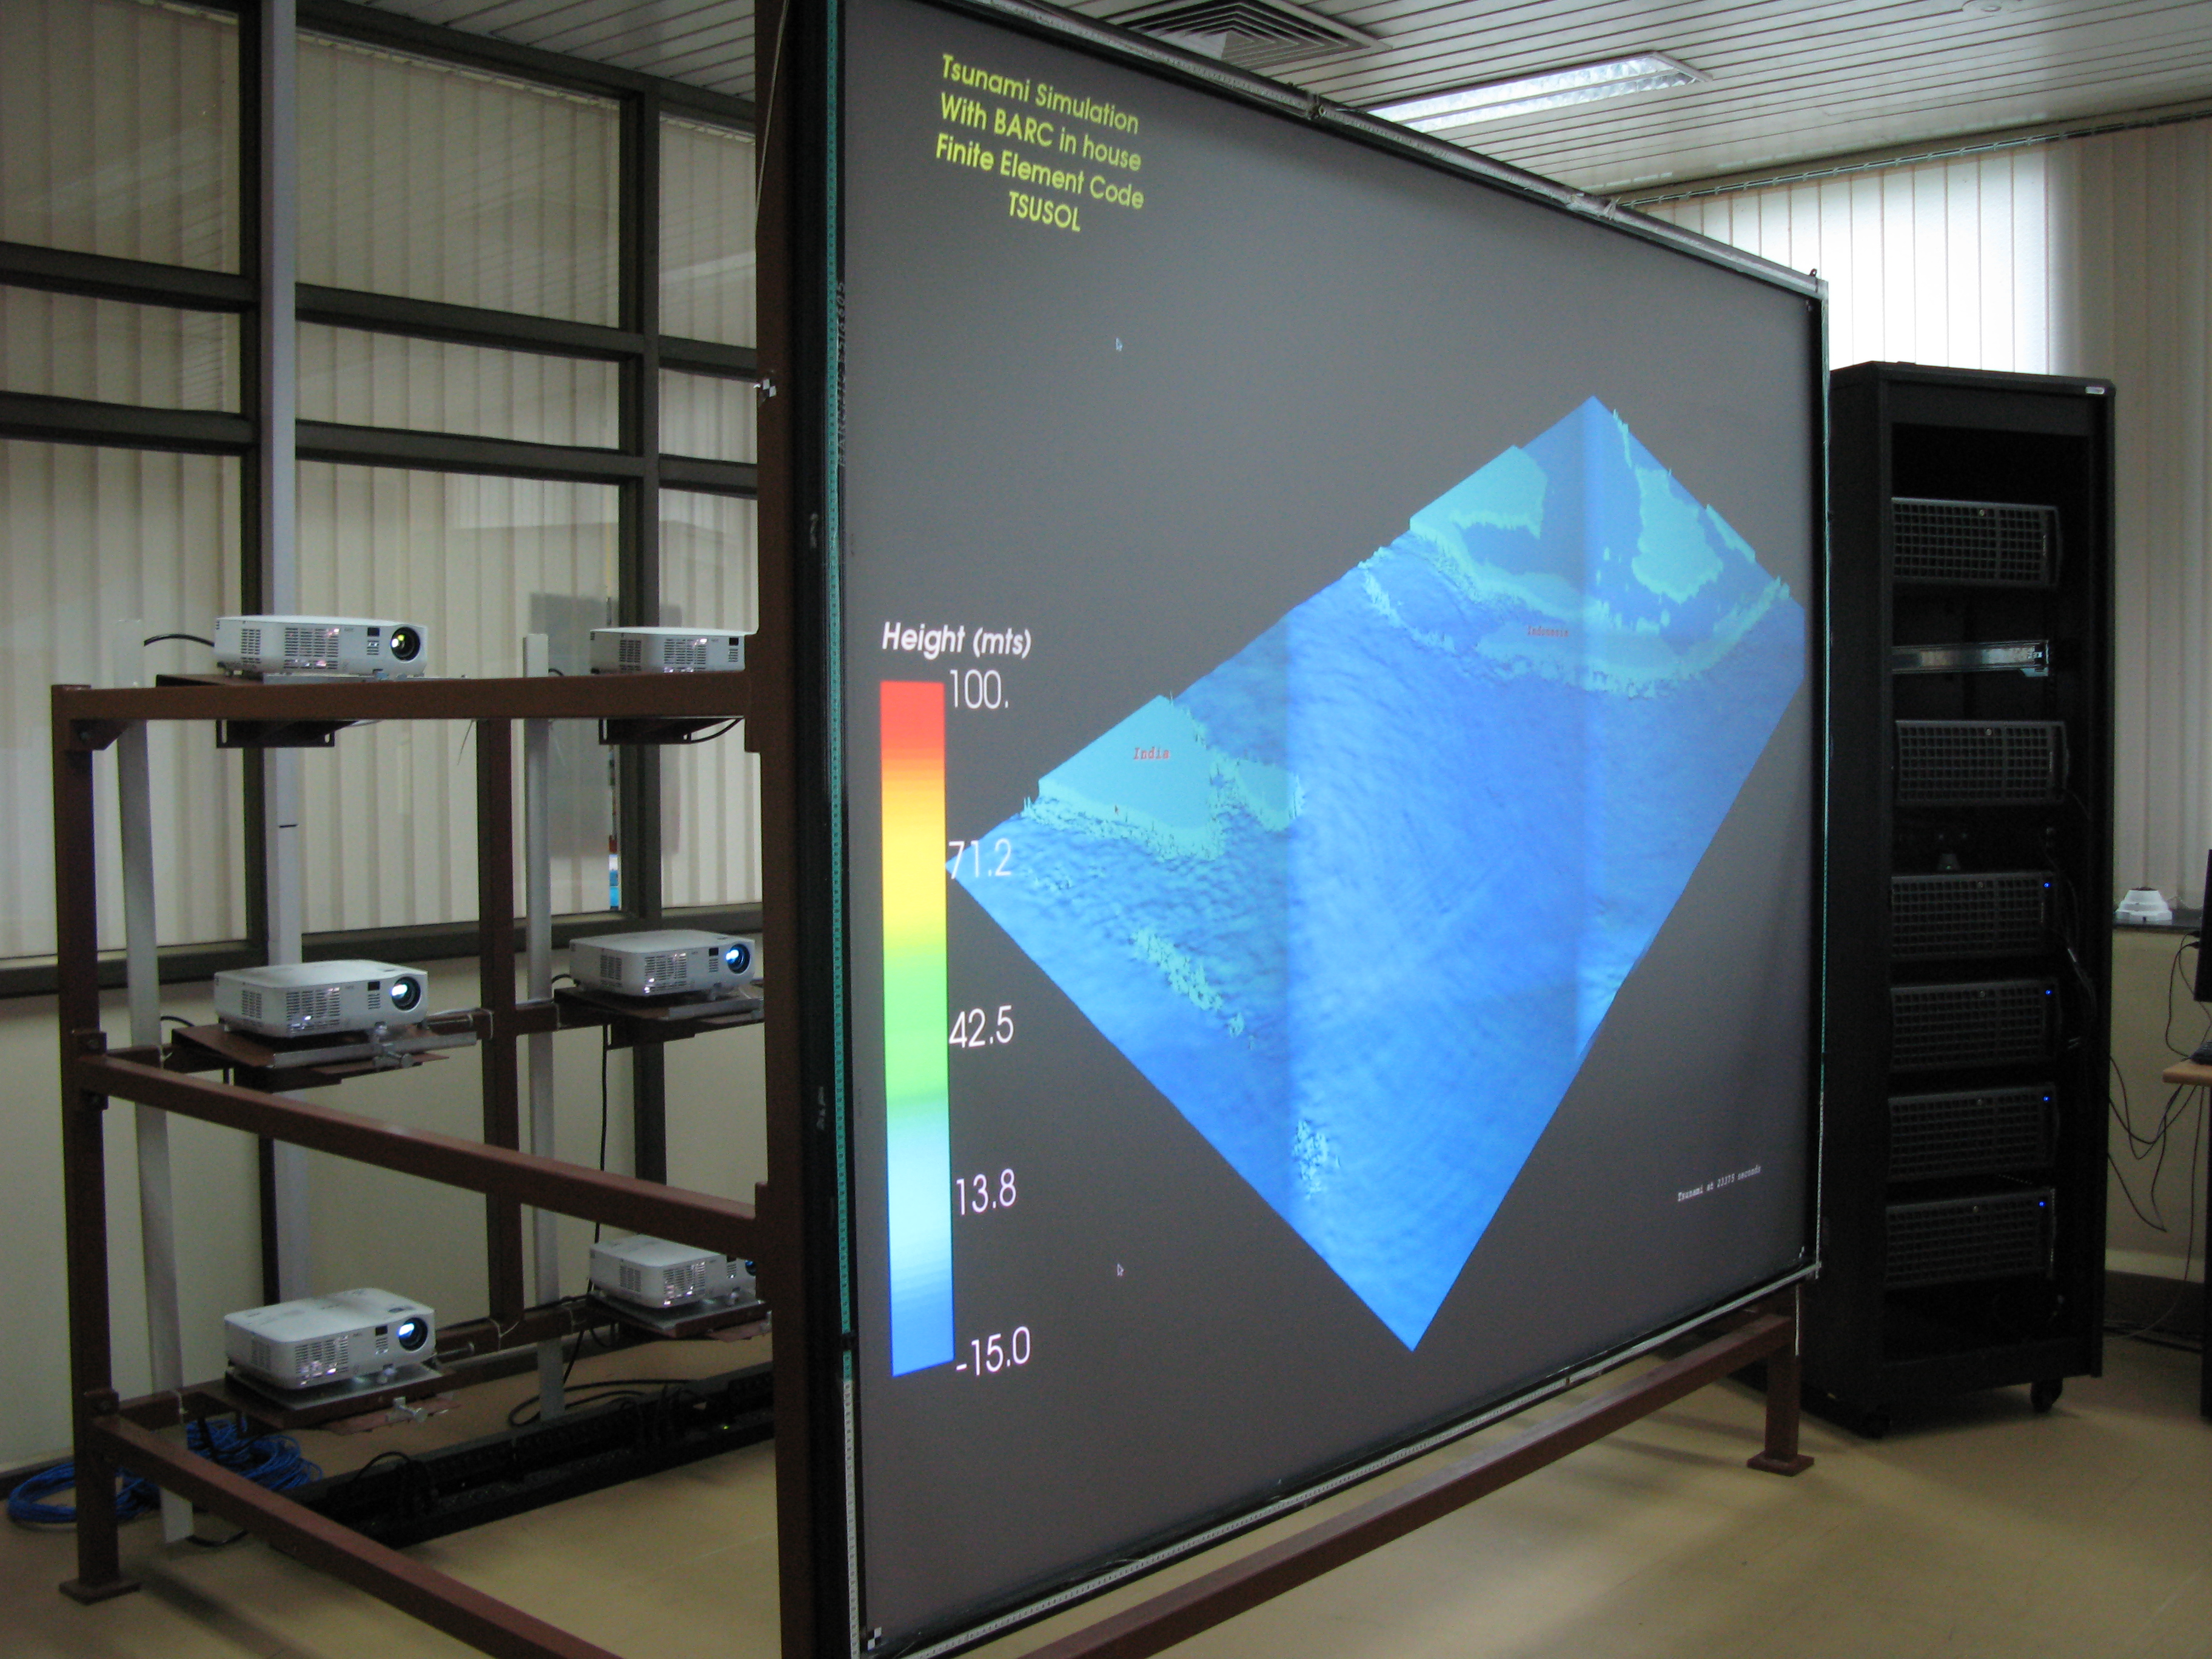
\includegraphics[width=4.5cm,height=3cm]{figures/system_setup.jpg}
\caption{Multiprojector tiled display}
\end{figure}

\end{frame}
%//////////////////////////////////////////////////////////////////////////////////////////////////////////////////////////////////

%//////////////////////////////////////////////////////////////////////////////////////////////////////////////////////////////////
\begin{frame}
\frametitle{Motivation}
\begin{enumerate}
\item Why \textit{Tiled}?\newline
An image with spatial resolution higher than that \textit{perceivable} by human eye cannot be visualized without reducing its resolution(So actually \textit{high megapixels} is just a marketing strategy, always check \textit{pixels per inch} instead). We can achieve this by spatially \textit{streching} the content.
\item Why \textit{Multiprojector}?\newline
Seams of monitors used in our earlier Tiled display system were \textit{distracting}. Projectors do not pose such limitation.
\end{enumerate}
\end{frame}

%//////////////////////////////////////////////////////////////////////////////////////////////////////////////////////////////////

\begin{frame}{Existing solutions}
\begin{enumerate}
\item Manual 
\item Automatic
\end{enumerate}
\end{frame}

%//////////////////////////////////////////////////////////////////////////////////////////////////////////////////////////////////

\begin{frame}{Why not a commercial system?}
\end{frame}

%//////////////////////////////////////////////////////////////////////////////////////////////////////////////////////////////////

\begin{frame}
\frametitle{Solution overview}
\begin{enumerate}
\item Geometric alignment
\begin{enumerate}
\item For each projector, determine distortion introduced by it  in the projected image on screen.
\item Apply inverse of this distortion to the projector image to recover geometrically continuos projection across neigboring projectors.
\end{enumerate}
\item Edge blending
\begin{enumerate}
\item Determine overlapping region between neighbouring projectors
\item Attenuate intensity of pixels in that region for all overlapping projectors so that their overlap does not create \textit{bright} junction between them
\end{enumerate}
\end{enumerate}
\end{frame}

%//////////////////////////////////////////////////////////////////////////////////////////////////////////////////////////////////


%//////////////////////////////////////////////////////////////////////////////////////////////////////////////////////////////////
\begin{frame}
\frametitle{System setup}
Developed system has:
\begin{enumerate}
\item 3X3 grid of projectors
\item Rear projection screen
\item 1 digital camera
\item Workstations arranged in Master-slave configuration
\end{enumerate}

\begin{figure}
\centering
\begin{tabularx}{\linewidth}{@{}cXX@{}}
\begin{tabular}{c c}
\hspace{0.5cm}\subfloat[System setup]{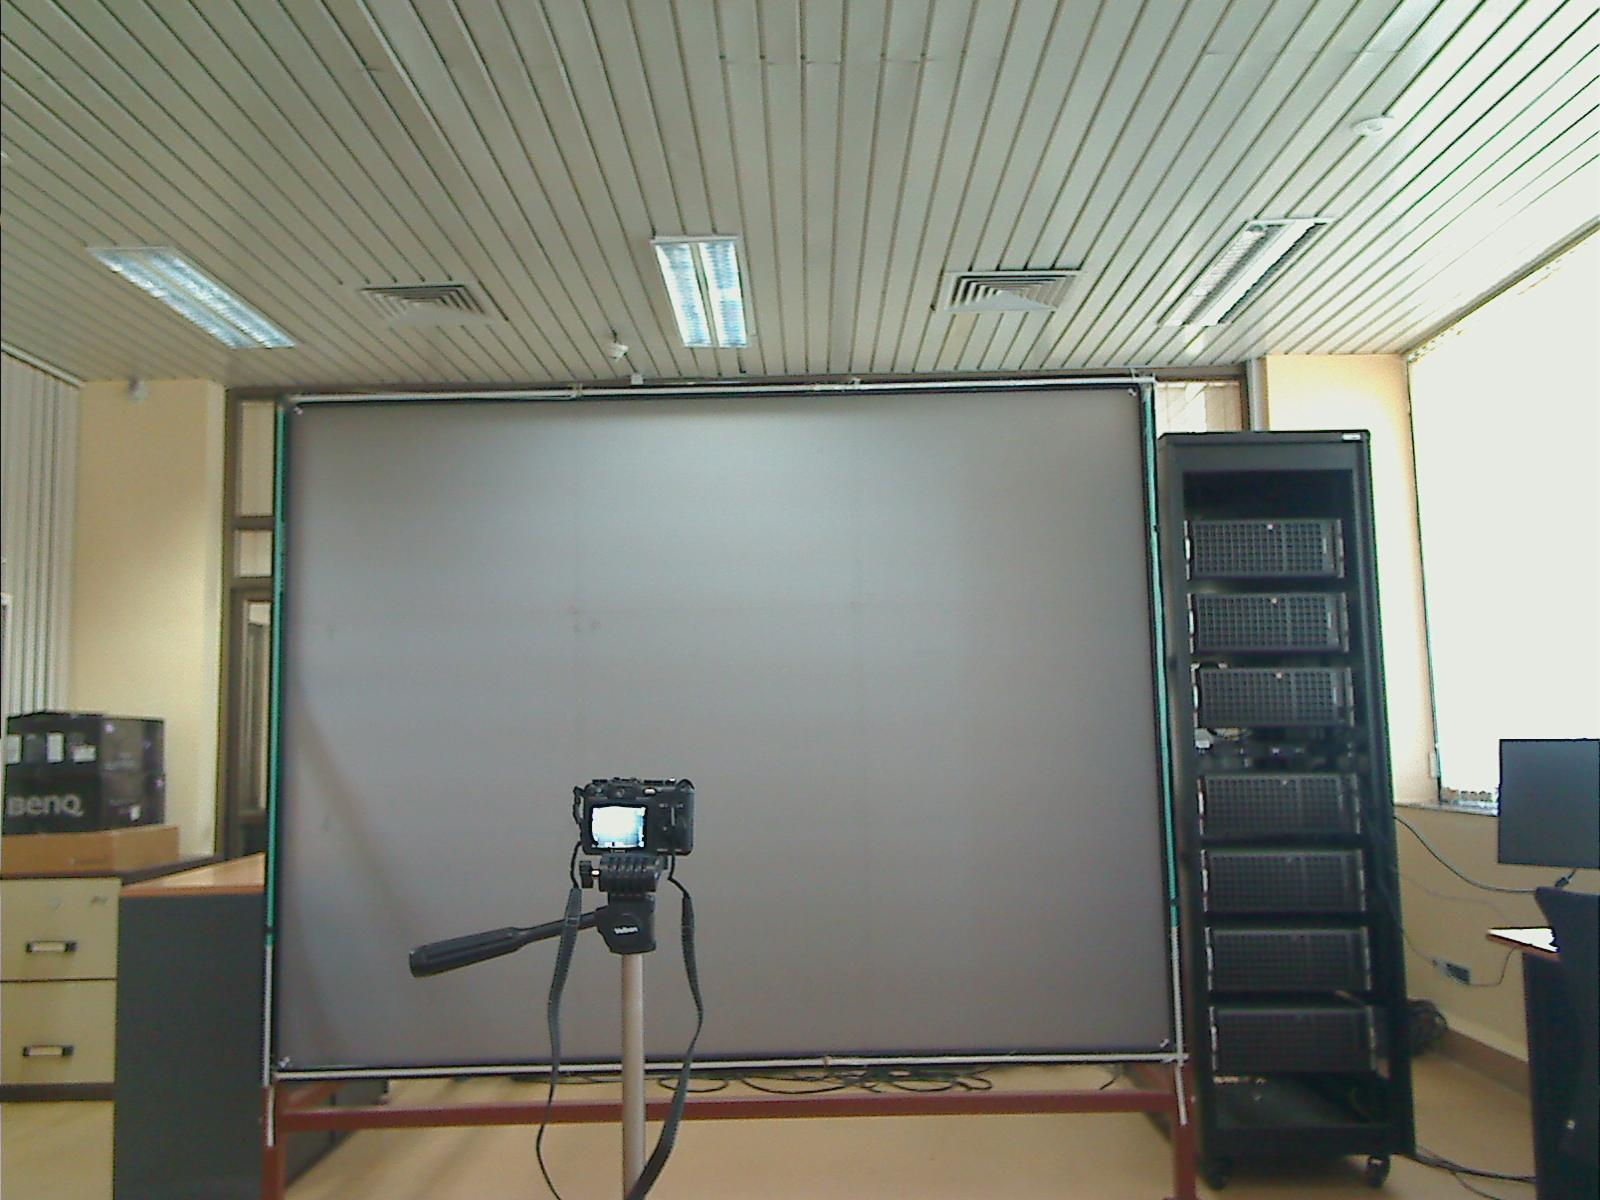
\includegraphics[width=4.5cm,height=3cm]{figures/setup.jpg}} & 
\subfloat[Projector-array behind the projection screen]{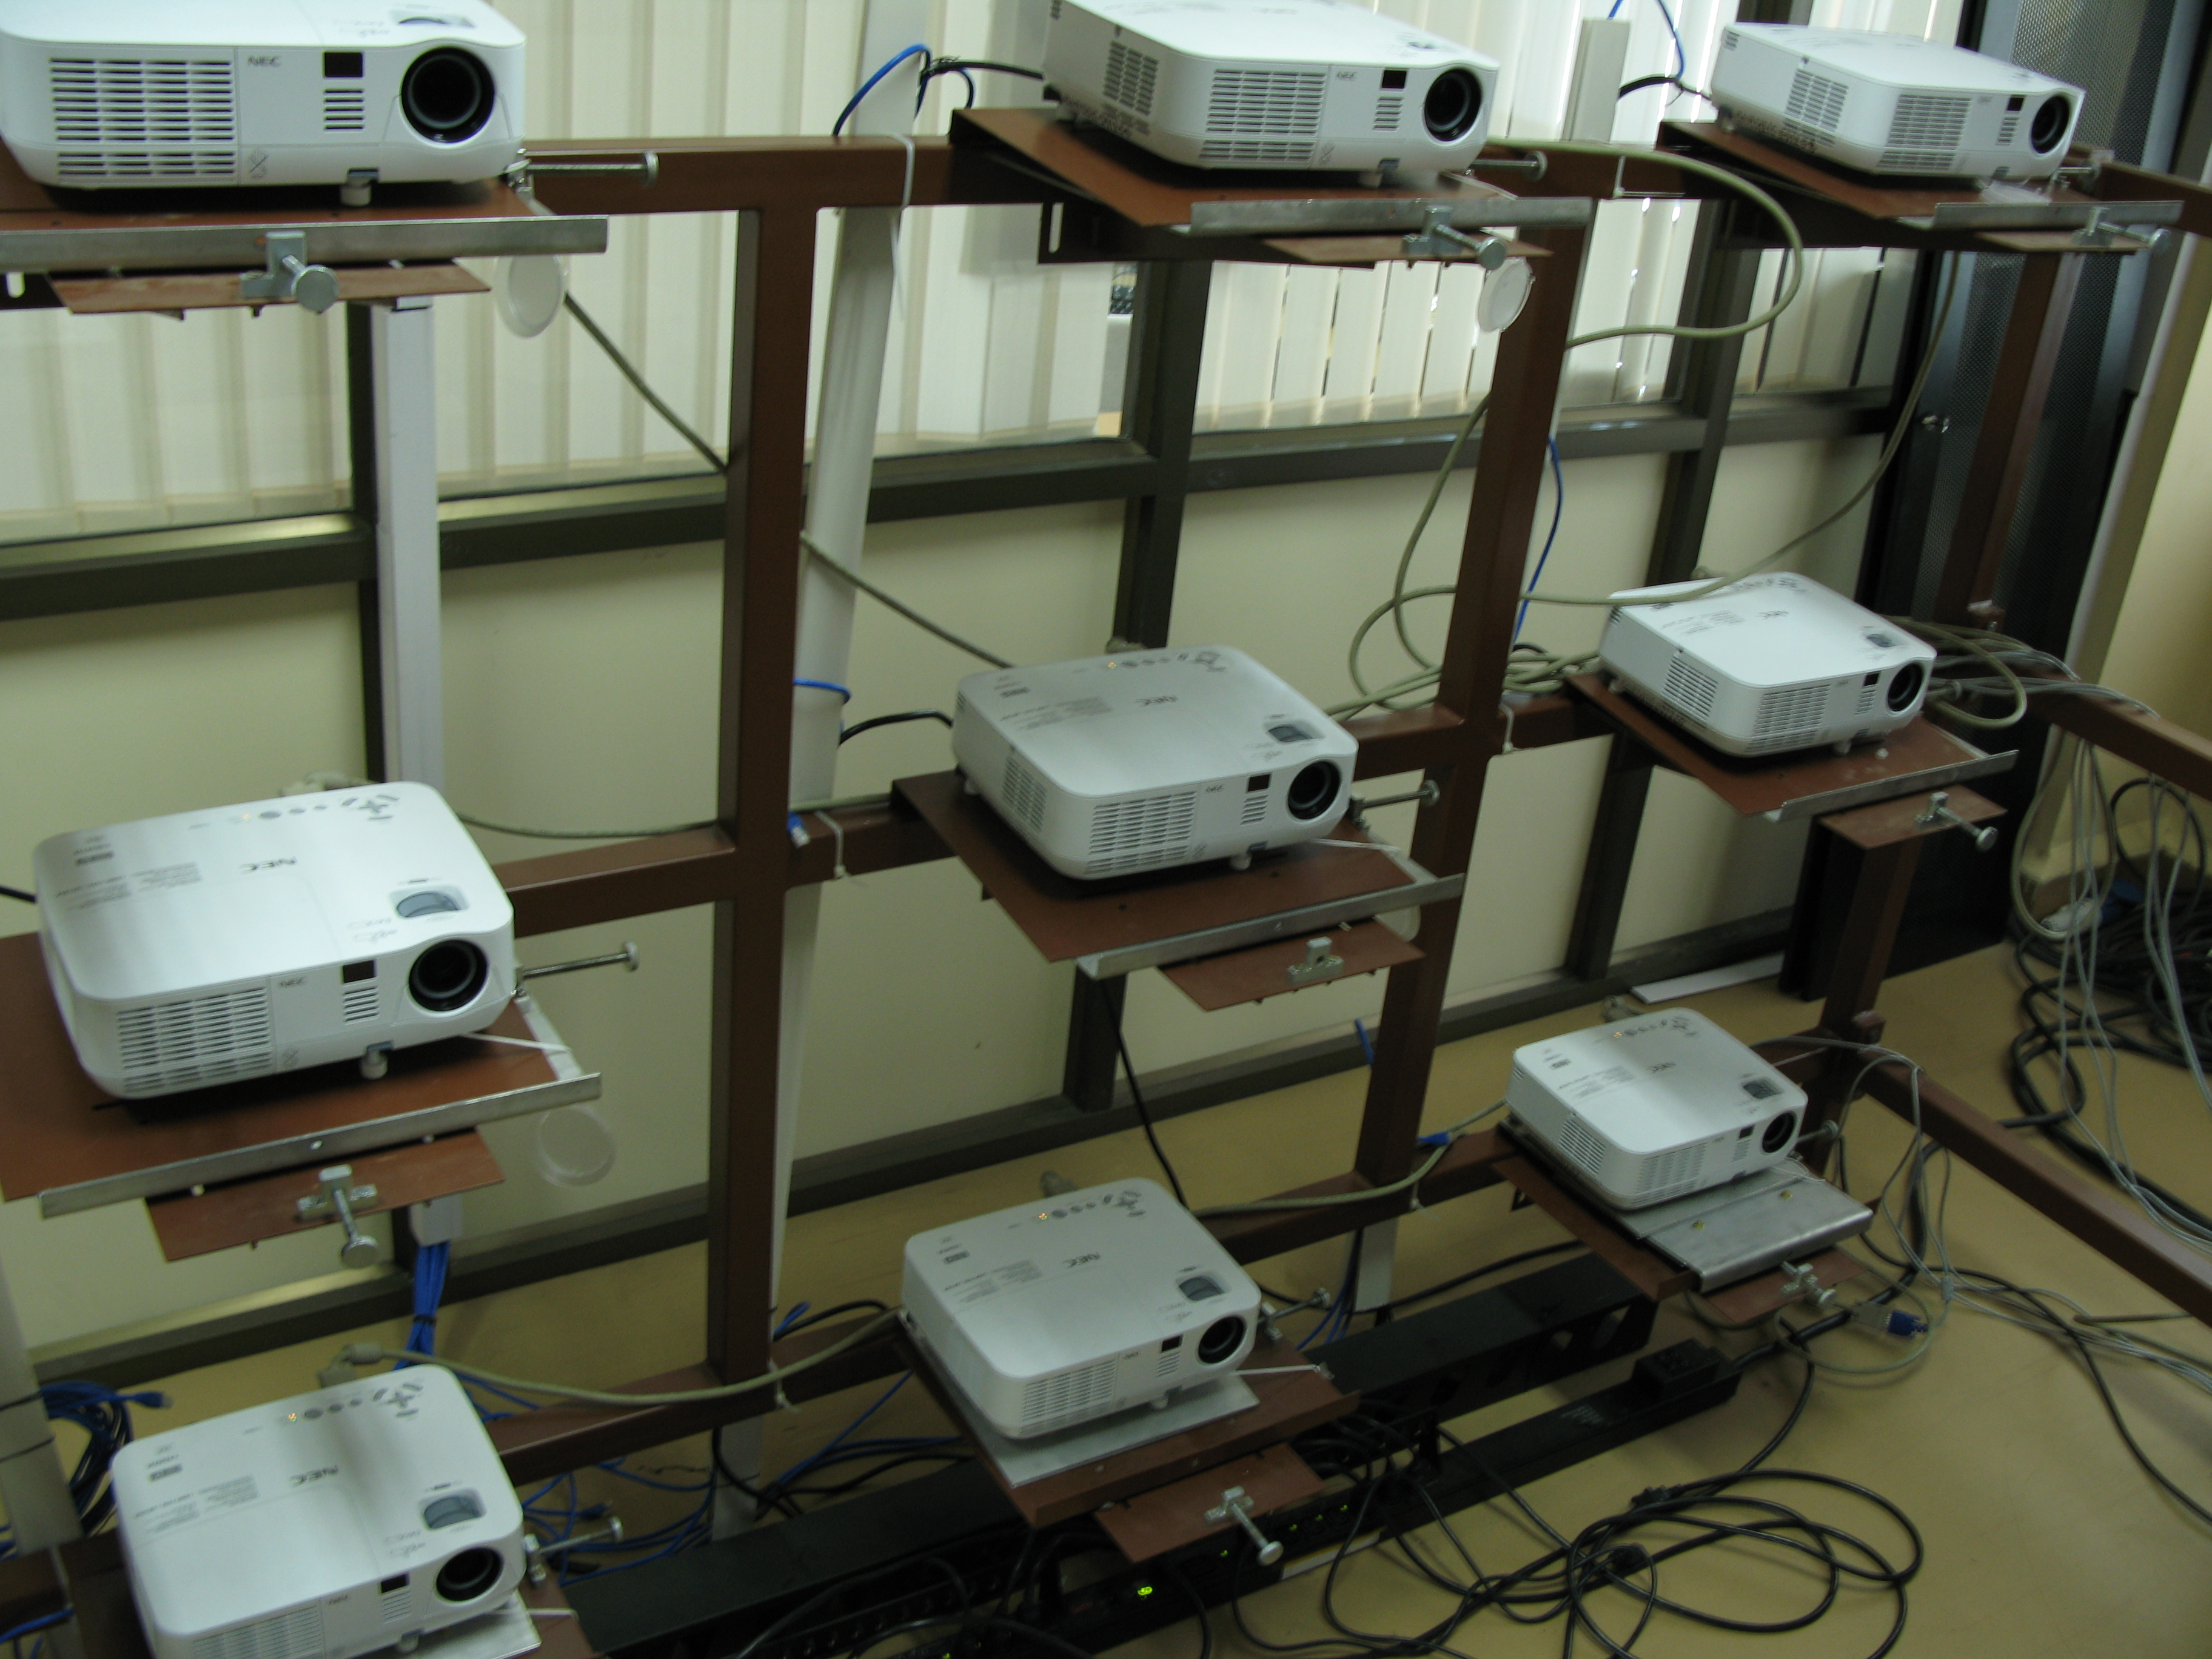
\includegraphics[width=4.5cm,height=3cm]{figures/projs.jpg}} \\
\end{tabular}
\end{tabularx}
\end{figure}

\end{frame}

%//////////////////////////////////////////////////////////////////////////////////////////////////////////////////////////////////
\begin{frame}
\frametitle{Algorithm}
\framesubtitle{Compute screen to camera relation}
\end{frame}
%//////////////////////////////////////////////////////////////////////////////////////////////////////////////////////////////////
\begin{frame}
\frametitle{Algorithm(contd.)}
\framesubtitle{Project and detect features for each projector}
Features are mapped to screen for subsequent computation.
\end{frame}
%//////////////////////////////////////////////////////////////////////////////////////////////////////////////////////////////////
\begin{frame}
\frametitle{Algorithm(contd.)}
\framesubtitle{Compute \textit{local} bounding boxes}
\end{frame}

\begin{frame}
\frametitle{Algorithm(contd.)}
\framesubtitle{Compute biggest \textit{local} bounding box}
\end{frame}


\begin{frame}
\frametitle{Algorithm(contd.)}
\framesubtitle{Compute \textit{global} bounding box}
\end{frame}

\begin{frame}
\frametitle{Algorithm(contd.)}
\begin{enumerate}
\item Compute normalized coordinate for detected features
\item Compute mapping between normalized \textit{projected} feature points and normalized \textit{detected} feature points
\item Compute position of local bounding boxes in the global bounding box
\item Compute alpha map
\end{enumerate}
\end{frame}

\begin{frame}
\frametitle{Novelity}
Cross-ratio based full projection region recovery
ADD FIGURE WITH CROSS RATIO WITOUT CROSS RATIO???????????
EQUATION OF CROSS RATIO???????????????????????????
\end{frame}

\begin{frame}
\frametitle{Results}
\begin{enumerate}
\item Software
\begin{enumerate}
\item Written in C
\item Dependent on OpenCV(v2.4.1) and libgphoto2(v2.5.2)
\item Works on Ubuntu(12.04 LTS) and Scientific Linux(6.1)
\end{enumerate}      
\item Hardware
\begin{enumerate}
\item 3X3 grid of NEC 200X DLP projectors
\item 2.4mX1.8m acyilic glass based rear projection screen(from ScreenTech,Germany)
\item Canon Powershot G7 digital camera
\item 4 Workstations(1 master+ 3 slave) with ???\newline
Each slave controls rendering on a row of projectors. It recieves rendering information from master using \textit{Chromium} framework.
\end{enumerate}
\end{enumerate}
\end{frame}

\begin{frame}
\frametitle{Results(contd.)}
\begin{enumerate}
\item Alignment procedure completes in 3-4 minutes as opposed to 30 mins. consumed in manual alignment approach
\item Proposed \textit{Cross ratio} based approach resulted in recovery of full projection region
\item Maximal misregistration between neighbouring projectors was around 2.5mm
SHOW FIGURE??????????????????
\item Paper selected for presentation at IEEE ICCCI-2014.
\end{enumerate}
\end{frame}


\begin{frame}
\frametitle{Issues}
View independent color seamless is still an \textit{open} problem
EMBEDD A VIDEO WITH VOICE SHOWING THE PROBLEM IN THE DISPLAY
\movie[]{Color seamlessness problem}{capture.avi}
\end{frame}



\end{document}
